\chapter{Simulations}


\section{Computational Domain}
\subsection{AMReX and Discretization}
Our target simulation is a 3D LES with a grid size that is 100 times the smallest scale of the turbulent flow. In our setup, the domain length in each direction is: $x = 25d$, $y = 62.5d$, and $z = 25d$, where the jet diameter $d=\SI{.01}{cm}$ and the $y$-axis is the axial direction of the jet. This smallest scale of these turbulent flows, known as the Kolmogorov scale \cite{kolmogorov}, can be approximated:
\begin{equation} \label{Kolmogorov}
	\eta = \left( \dfrac{\nu^3}{\varepsilon} \right)
\end{equation}
where $\nu = \nicefrac{\mu}{\rho}$ is the kinematic viscosity and $\varepsilon = \nicefrac{v_j^3}{d}$ is used to approximate the average rate of dissipation of turbulence kinetic energy per unit mass. For these turbulent jets, $\eta = \SI{5.37e-6}{cm}$. Therefore, to keep the calculation tractable and achieve an adequate \gls{les} grid size, we implement four levels of refinement, with a refinement ratio of 2, leading to 80, 200, and 80 cells on the coarsest level in the $x$, $y$, and $z$ directions, respectively. This results in an initial mesh size of $\Delta x_{0}=\Delta y_{0}=\Delta z_{0}=0.3125$, leading to $\Delta x_{3}=\Delta y_{3}=\Delta z_{3}=\SI{3.9062e-4}{}$, where the subscript denotes the \gls{amr} level. These four levels of refinement occur in the region outward from the jet inlet up to a distance of $20d$ in the $x$ and $z$ direction and $60d$ in the $y$ direction, as can be seen in Figure \ref{fig:domain}. The refinement criterion is given by the vorticity, specifically with $\omega \geq 5000^{2l}$, where $\omega$ is the magnitude of the vorticity and $l$ is the \gls{amr} level. For the first ten flow throughs of the simulation, mesh refinement only occurs up to one level within the refinement region to establish the flow pattern. Thereafter, the simulation proceeds  with the four levels of mesh refinement until reaching steady state, whereupon statistics are collected for analysis.
\begin{figure}[h!]
\centering
\begin{tikzpicture} [scale = .6]
	\draw [draw=c3med, fill=c3med!60, thick] (.5, 0) -- (4.5,0) -- (4.5, 12) -- (.5, 12) -- (.5, 0); 
	\draw [draw=c2med, fill=c2med!60, thick] (2.1, 0) -- (2.1, .4) -- (2.9, .4) -- (2.9, 0) -- (2.1, 0); 
	\draw [thick] (0,0) -- (5,0) -- (5,12.5) -- (0,12.5) -- (0,0);
	\draw [ultra thick] (2.4,0) -- (2.6, 0);
	\node [below] at (2.6,0) {\scriptsize{Jet Inlet}};
	\node [below] at (2.6,-.5) {\scriptsize{$v_j$, $T_j$}};
	\node [right] at (0.8, 10.4) {\scriptsize{Ambient Fluid}};
	\node [right] at (1.6, 9.9) {\scriptsize{$v_0 = 0$}};
	\node [right] at (1.6, 9.4) {\scriptsize{$T_0$, $p_0$}};
	\node [right] at (5, 6.25) {\footnotesize{$62.5d$}};
	\node [above] at (2.5, 12.5) {\footnotesize{$25d$}};
	%\node [below, c2med] at (.8, 2.2) {\tiny{4 levels}};
	%\node [below, c3med] at (6.25, .6) {\tiny{$\omega$ refinement}};
	\node [below] at (2.5, 12.6) {\scriptsize{Outflow BC}};
\end{tikzpicture}
\hspace{.1in}
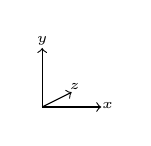
\begin{tikzpicture} [scale = .75]
	\draw [<->] (0,2.15) -- (0,1.15) -- (1,1.15);
	\draw[->] (0,1.15) -- (.5,1.4);
	\node [right] at (.85,1.175) {\tiny{$x$}};
	\node [right] at (.3, 1.5) {\tiny{$z$}};
	\node [above] at (0,2.025) {\tiny{$y$}};
\end{tikzpicture}
\caption{Two dimensional slice schematic of jet setup. Four levels of refinement are enforced within the green box based on proximity to jet inlet. Refinement based on vorticity criterion then occurs within the blue region. Outside the blue region, \gls{amr} is explicitly turned off to allow flow structures to be dissipated numerically and allowed to leave the domain without incurring spurious reflections.}
\label{fig:domain}
\end{figure}

\subsection{Initial and Boundary Conditions}
Our inlet consists of an opening centered in the $xz$-plane with diameter $d=\SI{.01}{cm}$ through which the \gls{sco2} jet is initialized. The pressure in the jet at the inlet is the same as that of the quiescent background fluid and it is given by $p_{j}=p_{0}=\SI{10.1325}{MPa}$. The ambient fluid remains at rest while the jet is initialized with an inflow velocity of $v_{j} = \SI{1800}{cm.s^{-1}}$, leading to a Reynolds number of the initialized jet of $Re_j = 22910$, with $v_{j}$ and $d$ being the reference velocity and length scale respectively. For the jet temperature and pressure conditions given, the reference density is $\rho_j=$ \SI{3.019e-1}{g.cm^{-3}}, as calculated via the \gls{srk} in \textit{PeleC}. To implement a turbulent inflow, we add noise to this input velocity using the mean velocity and \gls{rms} values from a predetermined \gls{dns} velocity profile \cite{DNS}. We begin by scaling the \gls{dns} values with our given jet velocity and radius. After determining which scaled \gls{dns} values we are near for the radius determined by our mesh, a linear interpolant is created to compute the mean velocity at our given radius. Noise is then added to each cylindrical component of the velocity as follows:
\begin{subequations} \label{Jet Inflow}
	\begin{align}
		v &= \langle v_{\text{\tiny{DNS}}} \rangle + \big(  v'_{\text{\tiny{DNS}}}  + \beta  v'_{\text{\tiny{DNS}}}    	r_1\sin{\theta_1}  \big) \cdot r_2 \sin{\theta_2} \label{y_flow} \\
		u &=   u'_{\text{\tiny{DNS}}}  + \beta  u'_{\text{\tiny{DNS}}}  r_3\sin{\theta_3} \label{t_flow} \\
		w &=   w'_{\text{\tiny{DNS}}}  + \beta  w'_{\text{\tiny{DNS}}}  r_4\sin{\theta_4}  \label{theta_flow}
	\end{align}
\end{subequations}  

\noindent where $\langle u_y \rangle$ is the mean velocity in the axial direction, $ u' = \langle u^2 \rangle^{\frac{1}{2}} $ is the \gls{rms} for each velocity component, and $\beta = 0.1$. Each $r_i$ and $\theta_k$ value is randomly generated as follows:
\begin{subequations} \label{Random_Variables}
	\begin{align}
		r_i &= \sqrt{-2.0 \log{(X_i)}} \label{Random_r} \\
		\theta_k &= 2 \pi X_k \label{Radom_theta}
	\end{align}
\end{subequations}

\noindent where $X_n$ are random numbers between 0 and 1. The inflow parameters are finalized after being converted into Cartesian coordinates.

We implement zero gradient boundary conditions for all boundaries not involving the jet inflow. Additionally, \gls{amr} is halted at a distance of $2.5d$ from the boundary in the $x$ and $z$ directions, and that of $5d$ in the axial direction in order to ensure that all waves are dissipated, thus avoiding spurious reflections from the boundaries. 

\section{Case Descriptions}
\subsection{Parameter Choices}
\section{Compute Time and Hardware Specifications}
\section{Post-Processing Procedures}




